\chapter{Discussion}

Our study indicates that the Provenance Replay software is likely
well-positioned for uptake by QIIME 2 users, and the core business requirements
sourced from the initial funding application have been met and exceeded. The
long-term success of this work, then, will likely rest on how well we can answer
the following questions:

\begin{itemize}
    \item How closely do study conditions mirror actual use?
    \item Have we met key non-functional requirements?
    \item How well does our work support in-silico reproducibility?
\end{itemize}

\section{Study vs field conditions}

With two major exceptions, the provenance replay demonstration component of our
study was fitted closely to likely user experience with the software in the
field. The demonstration was conducted in a natively installed QIIME 2
environment in a graphical Linux desktop environment, allowing familiar visual
interfaces for looking at and navigating file trees, and interacting with tools
like QIIME 2 View in the web browser. Some prospective provenance replay users will
primarily be interacting with QIIME 2 in headless cluster or server
environments. The command line interface for provenance replay was used as the
primary interface in the demonstration, to provide as much parity as possible
between these two experiences. Users of headless interfaces will have to manage
the same types of complexity for provenance replay that they do for standard
QIIME 2 analyses - transferring files to and from the cluster, reduced access to
contemporary code editing tools, and in some cases, insufficient permissions to
install software locally. 

This largely describes the standard overhead of working in a cluster
environment, and is not unique to Provenance Replay. For users who prefer to
work locally, most analytical steps in QIIME 2 can be performed in a reasonable
amount of time on a personal computer. The same is true for provenance replay,
which is capable of replaying a single Result in a few seconds, and a very large
analysis (450 results) in 8-10 minutes on a contemporary small-business laptop
(Intel Core i7-8565U CPU @ 1.8GHz, 16 GB RAM, OpenSUSE Tumbleweed running on an
M.2 SSD). As such, there is no practical requirement for normal users to work
with Provenance Replay in a cluster environment, and native installation is
recommended (and supported on Linux, MacOS, and Windows via the WSL2).

The other key difference between study conditions and current field conditions
lies in the installation process. Study participants were exposed to a QIIME 2
environment with Provenance Replay pre-installed for them, and were asked to
respond to questions under the explicit assumption that Provenance Replay was
packaged within their QIIME 2 environment. Software installation and management
can be a major challenge in the bioinformatics space, and Provenance Replay is
packaged to avoid the chief problems.

Integration with QIIME 2 is a long-term goal for this project, but the current
release is packaged separately, downloadable from a public repository hosted on
Github, and installable within a QIIME 2 conda environment with Python’s
\texttt{pip} \parencite{the_pip_developers_pip_2008}. This provides a “safe” and
uncluttered environment in which dependency conflicts can be managed actively.

As an interim solution on the road to integration, Provenance Replay will be
packaged for direct installation with conda \parencite{anaconda_inc_anaconda_2022},
providing a more robust environment solver and simplifying the installation
process for users of unix-like systems to a single easily-documented command.
Installation on Windows/WSL2 systems will still require the user to install
system dependencies, including WSL2, a linux instance on which QIIME 2 and
Provenance Replay can run, and conda, prior to running the install command. This
approach to packaging has worked well for QIIME 2, and many users of Provenance
Replay are likely to have these dependencies installed already, in support of
QIIME 2 itself.

Study conditions closely track real-world usage conditions for users of the
command line interface. (The Python API is not demonstrated.) Our demonstration
proceeds from an exercise in visualizing a provenance graph in q2view, through
the application of core replay features to single artifacts and to a
recursively-traversed directory structure. In-application documentation drives
discovery in the demonstration, and the documentation style is closely aligned
to the documentation style of QIIME 2 itself to keep things familiar. 

\section{Key non-functional requirements}

\subsection{Compatibility}

Provenance Replay is packaged for use across Linux, MacOS, and Windows (via
WSL2) using conda, which provides powerful dependency management and environment
solving tools. QIIME 2 versions \texttt{2021.11} and newer support Provenance
Replay, through their implementation of the Usage API and upstream usage drivers.
Results produced by any version(s) of QIIME 2 can be parsed and replayed.
Installing provenance replay within a clean QIIME 2 conda environment ensures
compatibility with the framework itself, and with many commonly used QIIME 2
plugins. Integration into the QIIME 2 framework, or placement in the QIIME 2
Library, will increase our ability to guarantee compatibility through access to
integration testing pipelines. Core dependencies of Provenance Replay were
selected with compatibility in mind, through a preference for well-maintained,
commonly-used, pure Python packages where appropriate.

\subsection{Permissive Error-Handling}

Because Provenance Replay targets both human and machine users, flexibility in
error handling is built into its primary interfaces. The \texttt{ChecksumValidator}
chooses to warn rather than raising errors, allowing human users to consider the
risks of invalid input data, while allowing replay to proceed without
interruption in automated processes. It may also be turned off, for users who do
not need it. Failures in parsing are raised as a custom \texttt{UnparseableDataError}
type, allowing API users to explicitly catch failures in parsing with a simple
\texttt{except} clause where appropriate.

\subsection{Licensing Requirements}

Like QIIME 2, Provenance Replay is released free of charge under the 3-clause
BSD license, which allows for public and private, commercial and non-commercial
use, modification, and distribution of the software. It offers no warranties of
fitness, and disclaims all liability. This license allows for broad use within
the field, and supports community development of the product and its ideas,
without exposing the developers to significant risks.

\subsection{Maintainability}

The most important of the non-functional requirements targeted here, this
software (and this thesis) were designed with maintainability in mind. On the
author’s graduation, maintenance of Provenance Replay will pass (in whole or in
part) to the QIIME 2 development team. To support their work, Provenance Replay
is written in Python 3 (the team’s core language), makes use of widely-used and
well-maintained libraries wherever possible, and attempts to minimize non-Python
dependencies. 

The Provenance Replay code base is unit tested to 100\% coverage, using
the \texttt{unittest} \parencite{python_software_foundation_unittest_2001} framework,
\texttt{pytest} \parencite{krekel_pytest_2015} as a test runner, and \texttt{pytest-cov} \parencite{pytest-cov_contributors_welcome_2016}
for coverage reporting. Automated testing is performed on all pull requests and
commits to the main branch, using GitHub actions
\parencite{github_features_2022} for continuous integration.

The code complies with PEP8 style guidelines \parencite{van_rossum_pep_2001}
which are enforced automatically with \texttt{flake8} during continuous integration,
imparting stylistic consistency with the QIIME 2 code base. The code is heavily
documented, using docstrings and in-line comments as necessary, in an effort to
provide both users and developers with the key information required to
understand the code and its rationale efficiently. Comments attempt to target
\textit{why} questions rather than \textit{what is happening here} questions
wherever possible, and best efforts have been made to write self-documenting
code with clear and descriptive naming conventions. Type annotations
are used throughout the code base, improving readability and allowing
maintainers to confirm the type-correctness of changes, without requiring them
to do so. \texttt{mypy} \parencite{lehtosalo_mypy_2014} has been used to verify
the correctness of these type annotations.

Special attention has been paid, as described above, to software extensibility
in areas where extensibility is known to be of benefit. Specifically, the parser
dispatch process, and the \texttt{ArchiveParser} version architecture are designed to
support simple extension, which we can reasonably expect will be necessary. 

Finally, the Future Work component of this document (chapter \ref{chapter:future_work})
is framed as a roadmap for next steps in the development and maintenance of
Provenance Replay. It is my hope that by outlining potential development targets
of value, I can set a strong foundation for the ongoing development of these
tools.


\subsection{Usability}

In the spirit of making reproducibility documentation “too easy not to do” \parencite[19]{whitaker_turing_2019},
usability is another key non-functional requirement. Users can generate
reproducibility supplements inline while working in either of QIIME 2’s most
popular user interface types. The command line interface targets usability by
exposing the minimum possible number of commands, adopting parameter naming
conventions familiar to QIIME 2 users, and providing sensible defaults that
allow commands to run with only input and output filepath parameters wherever
possible. Tab completion is enabled by default. The Python 3 API provides
slightly more flexibility (in line with the preferences of API users), but
exposes wrapper functions wherever appropriate that provide common workflows as
one-line commands. (Figure \ref{fig:simple_py_command})

\begin{figure}[htp]
\centering
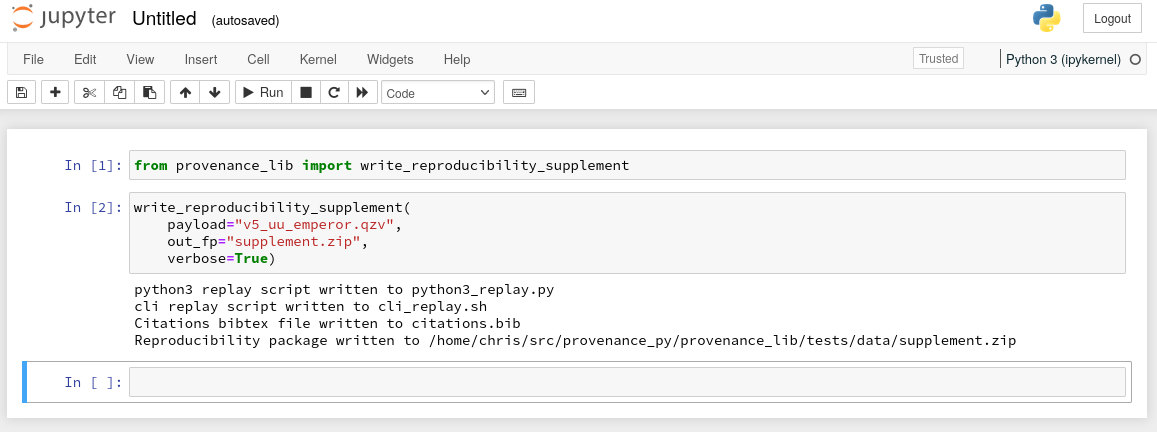
\includegraphics[width=\textwidth]{figures/supplement_replay_jn.png}
\caption[Screenshot of a simple Python 3 replay command]%
{Screenshot of a one-line wrapper command that parses provenance data and
writes a reproducibility supplement to disk. The command, shown within a
Jupyter Notebook, is passed required input and output filepath arguments, and
an optional argument to \texttt{verbose}. It generates scripts targeting all
supported interfaces and a bibtex-formatted citation library.}
\label{fig:simple_py_command}
\end{figure}

Help text is available from the command line or the Python interpreter, in
expected ways (e.g. \texttt{-–help} in the CLI and \texttt{?} in IPython).
Effort has been made to keep the installation process as simple as possible, and
high-level documentation supporting installation and basic use is available in
the repository \texttt{README} (See Appendices \ref{app:basicDocs} and
\ref{app:cliHelp}).

Finally, the Replay Usage drivers produce self-documenting outputs. For users
who intend to execute the scripts produced by Replay, step-by-step instructions
are written into script headers walking them through the process of doing so.


\section{Support for in-silico reproducibility}

Provenance Replay improves computational methods reproducibility in QIIME 2 by
reducing the practical overhead of important reproducibility outcomes. Framed in
terms of the user stories introduced in Section \ref{section:repro_goals},
provenance Replay supports:

\begin{itemize}
    \item Identification: a user can match UUIDs between replay outputs and the
        Results from which they were generated
    \item Validation: the \texttt{ChecksumValidator} confirms Result integrity
        against the MD5Sums captured when Results were first generated
    \item Reproduction: replay generates scripts that require only the input
        of original sample data for reproduction/corroboration of any original
        result (using captured sample metadata) when run in a compatible computing
        environment
    \item Extension/Generalization: replay generates executables that target
        extension to new data sets, sample metadata, and computing environments by
        flagging key inputs and changing parameter names for easy search
    \item Scaling/Automation: replay provides command options to increase
        permissiveness and/or improve runtime performance during parsing and replay
    \item Completeness: replay provides comprehensive access to all captured
        provenance data via an efficiently queryable \texttt{Networkx.Digraph}
        wrapped in a \texttt{ProvDAG} object. The Archive \texttt{Parser}s are architected
        with the goal of minimizing the cost of extension to accommodate additions
        to captured provenance.
\end{itemize}

Framed in terms of the “soft goals” for reproducibility from the same section (\ref{section:repro_goals}),
Provenance Replay targets the following with a high level of success.

\begin{itemize}
    \item Ease of Documentation: users can generate a complete “reproducibility
        package” including replay scripts and citation information with a single
        command, using their preferred user interface. Outputs (e.g. citations) are
        designed for interoperability with other common research tools where
        possible.
    \item Ease of Reproduction: replay scripts are executable with minimal
        modification, target a variety of interfaces, and are self-documenting,
        making them highly usable the first time.
    \item Ease of Automation: support for automation is limited at this time,
        but machine users have been considered in the architecture and design of
        provenance replay, and will be targeted in future development.
    \item Readability: replay documents are designed for humans, formatted
        nicely, and provide their own usage instructions.
    \item Learning-readiness: A variety of common interface-specific script
        output formats are provided, reducing interface-related barriers to
        readability and learning.
    \item Interpretation and communication: By providing multiple user
        interfaces for provenance replay, as well as multiple target interfaces for
        its outputs, users with varied computational skills can translate analyses
        for one another. Optional reporting of the metadata captured from the
        replayed study provides context for interpretation.
\end{itemize}

By implementing these features, Provenance Replay simplifies the process of
documenting research methods and attribution, while also making it easy to enact
and automate the reproduction of computational analyses. Further, it allows
users to interact with the computational history of any Result object(s) in
searchable and programmatic ways without requiring access to the original
script, notebook, or lab notes.

By providing variety in user interfaces available for the Provenance Replay
software itself, and in target user interfaces available for output scripts,
the software allows users to read and interact with these computational
histories through the familiar language of their preferred interface, improving
readability, reducing the technical cost of learning new methods, and lowering
barriers to interpretation and communication between users with different
technological backgrounds. By removing operational barriers to producing
reproducibility documentation, and by simplifying the enactment of reproduction
and extension, Provenance Replay allows QIIME 2 users the benefits of
reproducible science without many of the projected costs associated with
achieving reproducibility.

\section{First application in peer-reviewed microbiome research}

These tools have been applied to generate a reproducibility supplement for
publication with a large-scale analysis of relationships between Alzheimer’s
Disease pathology and the gut microbiome in transgenic mouse models that is
currently in peer review and available as a pre-print \parencite{borsom_predicting_2022}.
The supplement includes generated CLI and Python 3 scripts for reproducing the
analysis, full citations for a curated set of Result artifacts, and complete
sample metadata and raw data inputs. Scripts were updated to reference these
input data according to the machine-generated instructions. The instructions
were then simplified slightly by including third-party \texttt{.qza} inputs representing
a reference database and a pre-trained classifier in the package, and removing
the commands used to generate those Artifacts. The supplement will be published
to an open data repository, under embargo until paper publication, allowing
interested parties to more easily reproduce and build upon the published QIIME 2
analysis.
